Ограничения фильтрации методом скользящего среднего, связанные с невозможностью априорного задания параметров амплитудно-частотной характеристики, побуждают в ряде случаев применять другие методы проектирования цифровых фильтров.

В общем случае цифровой фильтр представляет собой линейную дискретную систему (рисунок~\ref{lab3_fig:structural_scheme}) с входным сигналом $x(n)$ и выходным сигналом $y(n)$, которая описывается уравнением

\begin{equation}
	\sum\limits_{m=1}^M a_m y (n-m) = \sum\limits_{k=1}^K b_k x (n-k),
	\label{lab3_eq:system}
\end{equation}

где $a_m, b_k$ – некоторые весовые коэффициенты, соответствующие отсчетам сигналов с номерами $m$ и $k$ соответственно.

\begin{figure}
	\centering
	\begin{tikzpicture}
	\draw (-2.75,1.75) -- (-2.75,3.15);
	\draw (-2.75,3.25) circle (0.1);
	\draw (-2.75,1.5) node {1};
	
	\draw (-2,1.75) -- (-2,2.9);
	\draw (-2,3) circle (0.1);
	\draw (-2,1.5) node {2};

	\draw (-1.25,1.75) -- (-1.25,3.65);
	\draw (-1.25,3.75) circle (0.1);
	\draw (-1.25,1.5) node {3};

	\draw (-0.5,1.75) -- (-0.5,2.4);
	\draw (-0.5,2.5) circle (0.1);
	\draw (-0.5,1.5) node {4};
	
	\draw[-latex] (-3.5,1.75) -- (0,1.75);
	\draw (0,0) -- (0,3.5) -- (3,3.5) -- (3,0) -- (0,0);
	\draw[-latex] (3,1.75) -- (6.5,1.752);
	
	\draw (3.5,1.75) -- (3.5,3.65);
	\draw (3.5,3.75) circle (0.1);
	\draw (3.5,1.5) node {1};
	
	\draw (4.25,1.75) -- (4.25,2.2);
	\draw (4.25,2.3) circle (0.1);
	\draw (4.25,1.5) node {2};
	
	\draw (5,1.75) -- (5,2.8);
	\draw (5,2.9) circle (0.1);
	\draw (5,1.5) node {3};
	
	\draw (5.75,1.75) -- (5.75,2.8);
	\draw (5.75,2.9) circle (0.1);
	\draw (5.75,1.5) node {4};
	
	\draw (-1.75,0.875) node {$x[n]$};
	\draw (1.5,1.75) node {$h[n]$};
	\draw (4.75,0.875) node {$y[n]$};
	
\end{tikzpicture}
	\caption{Структурная схема дискретной системы}
	\label{lab3_fig:structural_scheme}
\end{figure}

Используя \eqref{lab3_eq:system} получим выражение для текущего значения (с нулевой задержкой) выходного сигнала

\begin{equation}
	y(n) = \sum\limits_{k=0}^K \frac{b_k}{a_0}x(n-k) - \sum\limits_{m=1}^M \frac{a_m}{a_0}y(n-m).
	\label{lab3_eq:current}
\end{equation}

Таким образом, мы получили, что текущее значение выходного сигнала цифрового фильтра в общем случае определяется линейной комбинацией текущего входного значения сигнала, предыдущих отсчётов входного сигнала и предыдущих отсчётов выходного сигнала. Такой фильтр называется рекурсивным, так выходной сигнал зависит не только от входного, но и от предыдущих значений выходного сигнала.

В том случае, если $ \forall m > 0: a_m = 0 $, то выражение \eqref{lab3_eq:current} принимает вид

\begin{equation}
	y(n) = \sum\limits_{k=0}^K \frac{b_k}{a_0}x(n-k).
	\label{lab3_eq:current_v_2}
\end{equation}

Фильтр, описываемый выражением \eqref{lab3_eq:current_v_2}, называется нерекурсивным. Такое название подчеркивает, что выходной сигнал такого фильтра зависит только от отсчётов входного сигнала и не зависит от отсчётов выходного сигнала, а $h(k)$ представляет собой импульсную характеристкику нерекурсивного цифрового фильтра.

Используя понятие и обозначение свертки математического анализа \cite{ElementsOfAnalysis}, выражение \eqref{lab3_eq:current_v_2} можно переписать в виде

\begin{equation}
	y(n) = h(n) * x(n).
	\label{lab3_eq:convolution}
\end{equation}

Операция свертки является коммутативной, поэтому

\begin{equation}
	h(n) * x(n) = x(n) * h(n), \; a
	\label{lab3_eq:convolution_v_2}
\end{equation}

\begin{equation}
	\sum\limits_{k=0}^K h(k)x(n-k) = \sum\limits_{k=0}^K h(n-k)x(k)
	\label{lab3_eq:convolution_v_3}
\end{equation}

\emph{Импульсная характеристика фильтра} "--- это отклик фильтра при нулевых начальных условиях в виде выходной последовательности во временной области при подаче на вход единичного импульса.

Комплексной частотной характеристикой (КЧХ) $H_{\text{д}}(w)$ цифрового фильтра называется зависимость от частоты отношения комплексной амплитуды выходного дискретного гармонического сигнала к комплексной амплитуде входного дискретного гармонического сигнала в стационарном режиме. КЧХ определена

\begin{equation}
	H_{\text{д}}(w) = \frac{\dot Y}{\dot X},
	\label{lab3_eq:complex_frequency}
\end{equation}

и, как видно, является спектральной функцией для импульсивной характеристики $h_{\text{д}}(t)$.

Амплитудно-частотной характеристикой (АЧХ) $|H_{\text{д}}(w)|$ цифрового фильтра называется зависимость от частоты отношения амплитуды выходного дискретного гармонического сигнала к амплитуде входного дискретного гармонического сигнала в стационарном режиме:

\begin{equation}
	|H_{\text{д}}(w)| = \frac{Y}{X}
	\label{lab3_eq:frequency_response}
\end{equation}

Фазочастотной характеристикой (ФЧХ) $\varphi_{H_\text{д}} (w)$ цифрового фильтра называется зависимость от частоты разности начальных фаз выходного и входного дискретных гармонических сигналов в стационарном режиме

\begin{equation}
	\varphi_{H_{\text{д}}} (w) = \varphi_Y(w) - \varphi_X(w) = arg H_{\text{д}}(w).
	\label{lab3_eq:phase_response}
\end{equation}

Частотные характеристики цифрового фильтра являются переодическими функциями частоты с периодом $w_{\text{д}}$, однако, их чаще всего бывает удобно рассматривать как $2\pi$-переодические функции нормированной частоты $wT$ \cite{RadioChains}.

Примеры частотных характеристик приведены на рисунке~\ref{lab3_fig:types}.

\begin{figure}
	\centering
	\scalebox{.85}{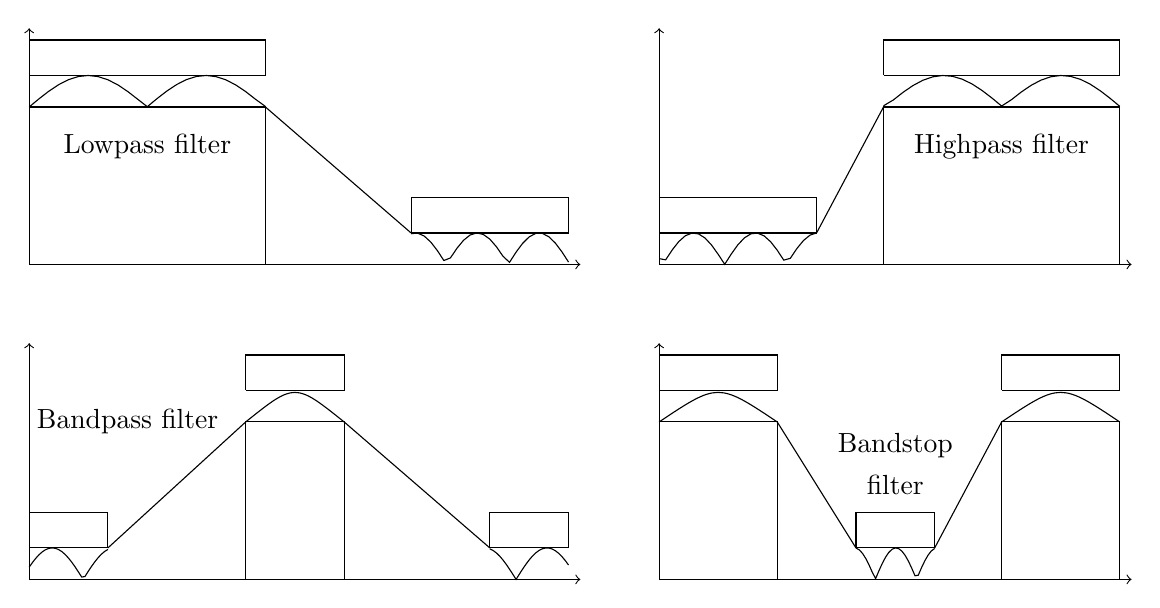
\begin{tikzpicture}
	\draw[->] (0,0) -- (0,3);
	\draw[->] (0,0) -- (7,0);
	
	\draw (0,2.4) -- (0,2.85) -- (3,2.85) -- (3,2.4) -- (0,2.4);
	\draw (0,0) -- (0,2) -- (3,2) -- (3,0) -- (0,0);
	\draw (4.85,0.4) -- (4.85,0.85) -- (6.85,0.85) -- (6.85,0.4) -- (4.85,0.4);
	
	\draw[->] (0,-4) -- (0,-1);
	\draw[->] (0,-4) -- (7,-4);
	
	\draw (0,-3.6) -- (0,-3.15) -- (1,-3.15) -- (1,-3.6) -- (0,-3.6);
	\draw (2.75,-1.6) -- (2.75,-1.15) -- (4,-1.15) -- (4,-1.6) -- (2.75,-1.6);
	\draw (2.75,-4) -- (2.75,-2) -- (4,-2) -- (4,-4) -- (2.75,-4);
	\draw (5.85,-3.6) -- (5.85,-3.15) -- (6.85,-3.15) -- (6.85,-3.6) -- (5.85,-3.6);
	
	\draw[->] (8,0) -- (8,3);
	\draw[->] (8,0) -- (14,0);
	
	\draw (8,0.4) -- (8,0.85) -- (10,0.85) -- (10,0.4) -- (8,0.4);
	\draw (10.85,2.4) -- (10.85,2.85) -- (13.85,2.85) -- (13.85,2.4) -- (10.85,2.4);
	\draw (10.85,0) -- (10.85,2) -- (13.85,2) -- (13.85,0) -- (10.85,0);
	
	\draw[->] (8,-4) -- (8,-1);
	\draw[->] (8,-4) -- (14,-4);
	
	\draw (8,-1.6) -- (8,-1.15) -- (9.5,-1.15) -- (9.5,-1.6) -- (8,-1.6);
	\draw (8,-4) -- (8,-2) -- (9.5,-2) -- (9.5,-4) -- (8,-4);
	\draw (10.5,-3.6) -- (10.5,-3.15) -- (11.5,-3.15) -- (11.5,-3.6) -- (10.5,-3.6);
	\draw (12.35,-1.6) -- (12.35,-1.15) -- (13.85,-1.15) -- (13.85,-1.6) -- (12.35,-1.6);
	\draw (12.35,-4) -- (12.35,-2) -- (13.85,-2) -- (13.85,-4) -- (12.35,-4);
	
	\draw[domain=0:3] plot (\x, {2 + abs(0.4*sin(2.1*\x r))});
	\draw (3,2) -- (4.85,0.4);
	\draw[domain=4.85:6.85] plot (\x, {abs(0.4*sin(4*(\x+0.20) r))});
	 
	\draw[domain=0:1] plot (\x, {abs(0.4*sin(4*(\x+0.10) r)) - 4});
	\draw (1,-3.6) -- (2.75,-2);
	\draw (2.75,-2) .. controls (3.375,-1.5) .. (4,-2);
	\draw (4,-2) -- (5.85,-3.6);
	\draw[domain=5.85:6.85] plot (\x, {abs(0.4*sin(4*(\x+0.10) r)) - 4});
	 
	\draw[domain=8:10] plot (\x, {abs(0.4*cos(4*(\x+0.20) r))});
	\draw (10,0.4) -- (10.85,2);
	\draw[domain=10.85:13.85] plot (\x, {2 + abs(0.4*sin(2.1*(\x+1.1) r))});
	
	\draw (8,-2) .. controls (8.75,-1.5) .. (9.5,-2);
	\draw (9.5,-2) -- (10.5,-3.6);
	\draw[domain=10.5:11.5] plot (\x, {abs(0.4*sin(6*(\x+0.25) r)) - 4});
	\draw (11.5,-3.6) -- (12.35,-2);
	\draw (12.35,-2) .. controls (13.1,-1.5) .. (13.85,-2);
	
	\draw (1.5,1.5) node {Lowpass filter};
	\draw (12.35,1.5) node {Highpass filter};
	\draw (1.25,-2) node {Bandpass filter};
	\draw (11,-2.3) node {Bandstop};
	\draw (11,-2.8) node {filter};
\end{tikzpicture}}
	\caption{Основные типы амплитудно-частотных характеристик цифровых фильтров}
	\label{lab3_fig:types}
\end{figure}

Нерекурсивный фильтр в отличие от рекурсивного всегда:

\newcounter{c}[section]

\setcounter{c}{1} \arabic{c}. Имеет конечную импульсную характеристику.\par
\setcounter{c}{2} \arabic{c}. Имеет линейную фазо-частотную характеристику.\par
\setcounter{c}{3} \arabic{c}. Является устойчивым.\par

Линейная фазо-частотная характеристика обеспечивает равномерную задержку всех гармоник сигнала вне зависимости от значения их частоты.

Фильтр называется \emph{устойчивым}, если при любых конечных начальных условиях и любом ограниченном входном сигнале выходной сигнал также остается ограниченным.